%%%%%%%%%%%%%%%%%%%%%%%%%%%%%%%%%%%%%%%%%%%%%%%%%%%%%%%%%%%%%%%%%%%%%%%%%%%%
%%                                                                        %%
%%                 Support de cours Programmation orientée objet                  %%
%%                                                                        %%
%%%%%%%%%%%%%%%%%%%%%%%%%%%%%%%%%%%%%%%%%%%%%%%%%%%%%%%%%%%%%%%%%%%%%%%%%%%%
%% Guillaume Moreau (EC Nantes)
%% création : 21/06/2004
%% dernière modification : 23/06/2004
%% historique :

%% il faut fixer l'URL base pour que les liens relatifs fonctionnent...
%% bizaremment fichu mais c'est comme ça.

\documentclass[allowframebreaks,xcolor=dvipsnames]{beamer}

\mode<presentation>
{
\usetheme{Antibes}
  % or ...

  %\setbeamercovered{transparent}
  % or whatever (possibly just delete it)
}
\useoutertheme{infolines}
\usecolortheme[named=RoyalBlue]{structure}

\uselanguage{french}
\languagepath{french}
\deftranslation[to=french]{definition}{définition}
\deftranslation[to=french]{Definition}{D\'efinition}
\deftranslation[to=french]{example}{exemple}
\deftranslation[to=french]{Example}{Exemple}
\deftranslation[to=french]{algorithm}{algorithme}
\deftranslation[to=french]{Algorithm}{Algorithme}

\setbeamertemplate{blocks}[rounded][shadow=true]
\setbeamertemplate{navigation symbols}{}
\setbeamertemplate{itemize item}[square]
\setbeamertemplate{itemize subitem}[triangle]

\usepackage[T1]{fontenc}
% or whatever

\usepackage[french]{babel}
% or whatever

\usepackage{tikz}
\usetikzlibrary{graphs}
\usetikzlibrary{graphdrawing.force}
\usetikzlibrary{arrows}
\usepackage{tikz-network}

%% pour afficher le plan à chaque début de section
%\AtBeginSection[]{
%  \begin{frame}{Plan}
%  \tiny \tableofcontents[currentsection, hideothersubsections]
%  \end{frame}
%}


%% tout ce qui est relatifs aux extraits de code
\usepackage{minted}
\newminted{python}{fontsize=\footnotesize}


\usepackage{myslides}

%% mes styles pour les graphes
\usepackage{graphstyle}

%\usepackage{times}
\usepackage[T1]{fontenc}
% Or whatever. Note that the encoding and the font should match. If T1
% does not look nice, try deleting the line with the fontenc.


\title[Option INFO / MADIS] % (optional, use only with long paper titles)
{Mathématiques discrètes : algorithmique des graphes}

\author[G. Moreau]{Guillaume Moreau\\
\texttt{guillaume.moreau@ec-nantes.fr}}
% - Use the \inst{?} command only if the authors have different
%   affiliation.

\institute[Ecole Centrale de Nantes] % (optional, but mostly needed)
{
  Ecole Centrale de Nantes
}

\date % (optional)
{Septembre 2020}

\subject{Théorie et algorithmique des graphes}


\definecolor{webgreen}{rgb}{0,.5,0}
\definecolor{webbrown}{rgb}{.6,0,0}
\definecolor{* }{rgb}{0,.5,0}
\definecolor{. }{rgb}{.6,0,0}

% option d'affiche de table des matières : http://mirror.unl.edu/ctan/macros/latex/contrib/beamer/doc/beameruserguide.pdf
% section 10.5

% Delete this, if you do not want the table of contents to pop up at
% the beginning of each subsection:
\AtBeginSection[]
{
   \begin{frame}
       \frametitle{Plan}
       \tableofcontents[sectionstyle=show/hide,subsectionstyle=show/show/hide,subsubsectionstyle=hide/hide]
   \end{frame}
}

\AtBeginSubsection[]
{
	\begin{frame}
		\frametitle{Plan}
		\tableofcontents[sectionstyle=show/hide,subsectionstyle=show/shaded/hide,subsubsectionstyle=show/show/hide]
	\end{frame}
}

\begin{document}

\begin{frame}
  \titlepage
\end{frame}

\begin{frame}[allowframebreaks]{Plan du cours}
  \tableofcontents[hideallsubsections]
  % You might wish to add the option [pausesections]
\end{frame}

% TODO ajouter un index


% Algorithmes de flot max
\section{Corrigé TD flot max}
\begin{frame}{Variante de l'algorithme de Ford \& Fulkerson}
    \begin{itemize}
        \item L'algorithme vu en cours est efficace mais peu évident à appliquer \emph{visuellement}
        \item On peut modifier la recherche de chaine augmentante sans utiliser le graphe résiduel
        \item Principe 
        \begin{itemize}
            \item Repérer les chaines augmentantes \emph{de visu} et augmenter le flot en conséquence 
            \item Utiliser un simple algorithme de marquage pour repérer de nouvelles chaines augmentantes
        \end{itemize}
    \end{itemize}
\end{frame}

\begin{frame}{Recherche de chaine augmentante}
\begin{tabbing}
    \= xx \= xx \= xx \= xx \= xx \=
    xxxxxxxxxxxxxxxxxxxxxxxxxxxxxxxxxxxxxxxxxxxxxxxxxxx\kill
    \> Soit $x$ un flot admissible, marquer \textbf{+} le sommet $s$ \\
    \> \textbf{Répéter} \\
    \> \> \textbf{Si} $i$ est marqué et $j$ non marqué \textbf{Alors} \\
    \> \> \> \textbf{Si} $(i,j)$ est un arc non saturé \textbf{Alors} \\
    \> \> \> \> marquer $j$ avec \textbf{+} \\
    \> \> \> \textbf{FinSi} \\
    \> \> \> \textbf{Si} $(j,i)$ est un arc tel que $x_{ij} > 0$  \textbf{Alors} \\
    \> \> \> \> marquer $j$ avec \textbf{-} \\
    \> \> \> \textbf{FinSi} \\
    \> \> \textbf{FinSi} \\
    \> \textbf{Jusqu'à} ce qu'on ne puisse plus marquer de sommets \\
    \> \textbf{Si} $t$ est marqué \textbf{Alors} \\
    \> \> il existe une chaîne augmentante de $s$ à $t$ \\
    \> \> augmenter le flot et recommencer \\
    \> \textbf{Sinon} \\
    \> \> le flot est maximal \\
    \> \textbf{FinSi} \\
  \end{tabbing}

  
\end{frame}

\begin{frame}{graphe initial}
        \begin{center}
            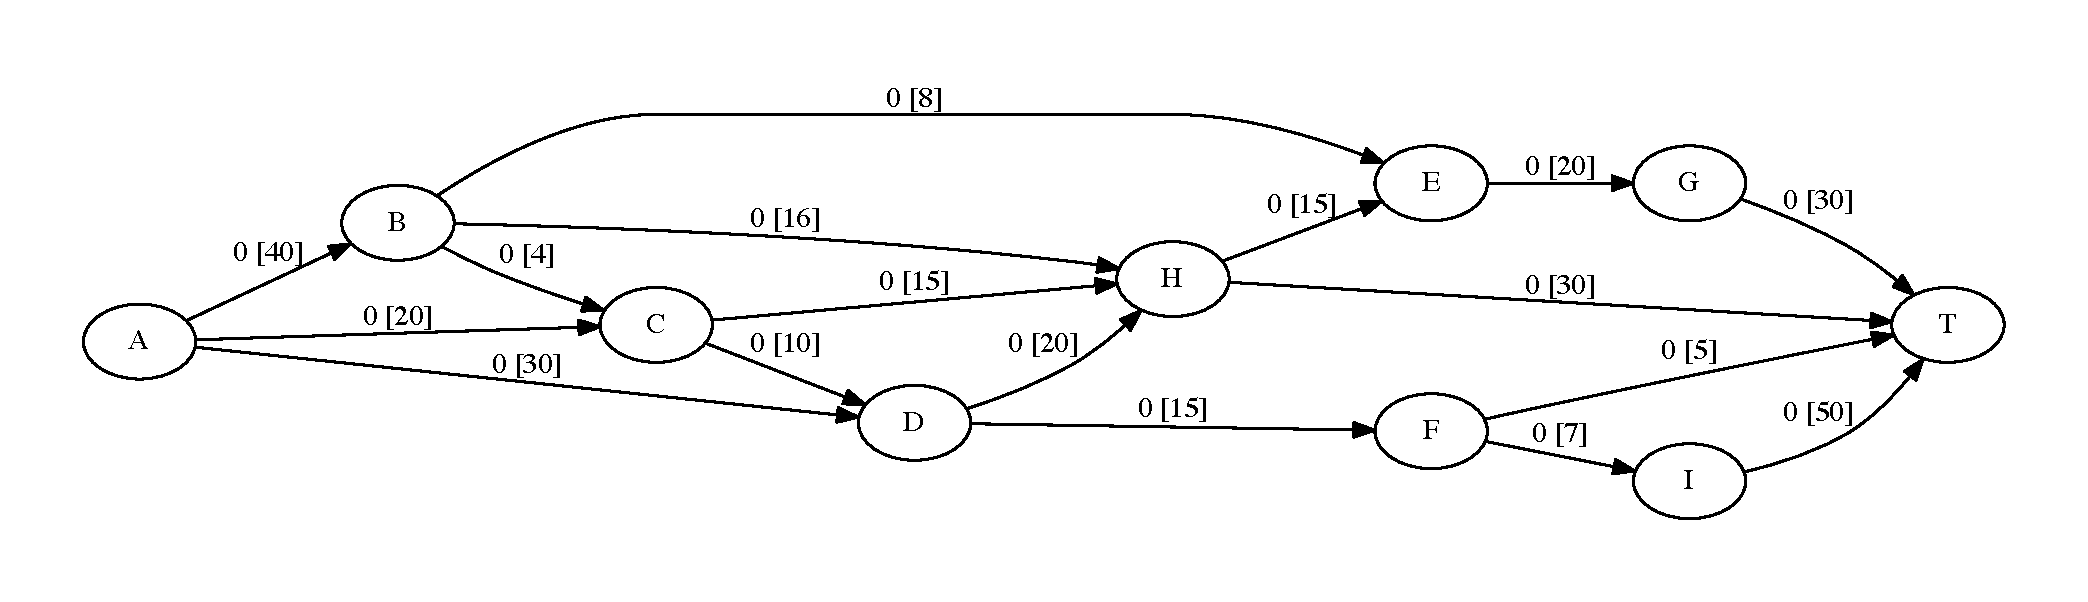
\includegraphics[width=\textwidth]{tutorials/pcc/figs/reseau.pdf}
        \end{center}
        
        
\end{frame}

\begin{frame}{}
    On choisit une première chaîne augmentante : A-B-H-T, on peut augmenter le flot du minimum des capacités, soit 16.
    \begin{center}
        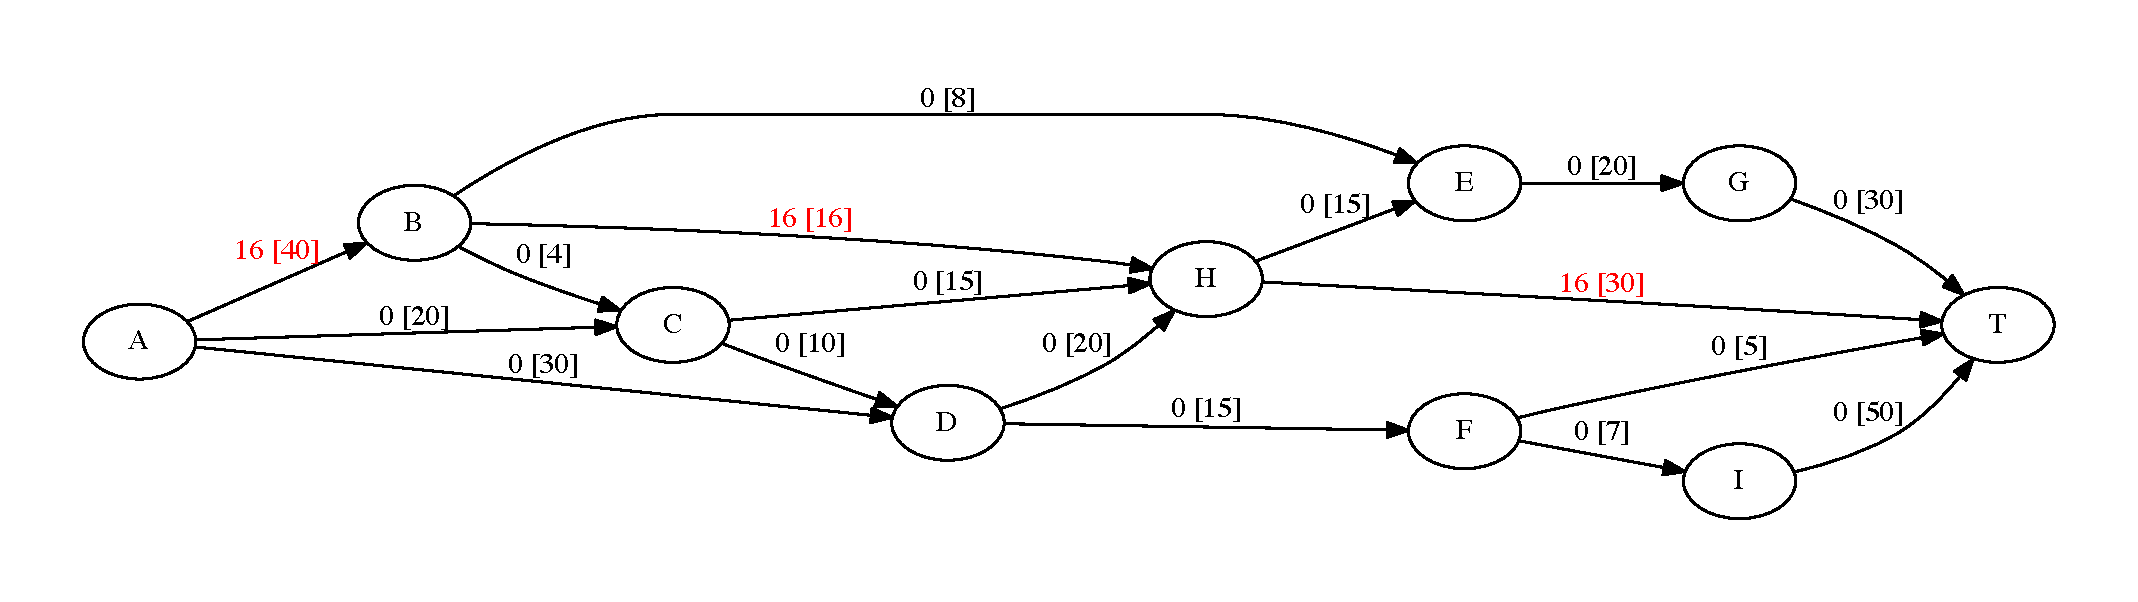
\includegraphics[width=\textwidth]{tutorials/pcc/figs/reseau-1.pdf}
    \end{center}
\end{frame}

\begin{frame}{}
    On choisit ensuite une seconde chaîne augmentante, A-D-F-I-T qui permet d'augmenter le flot de 7.    
    \begin{center}
        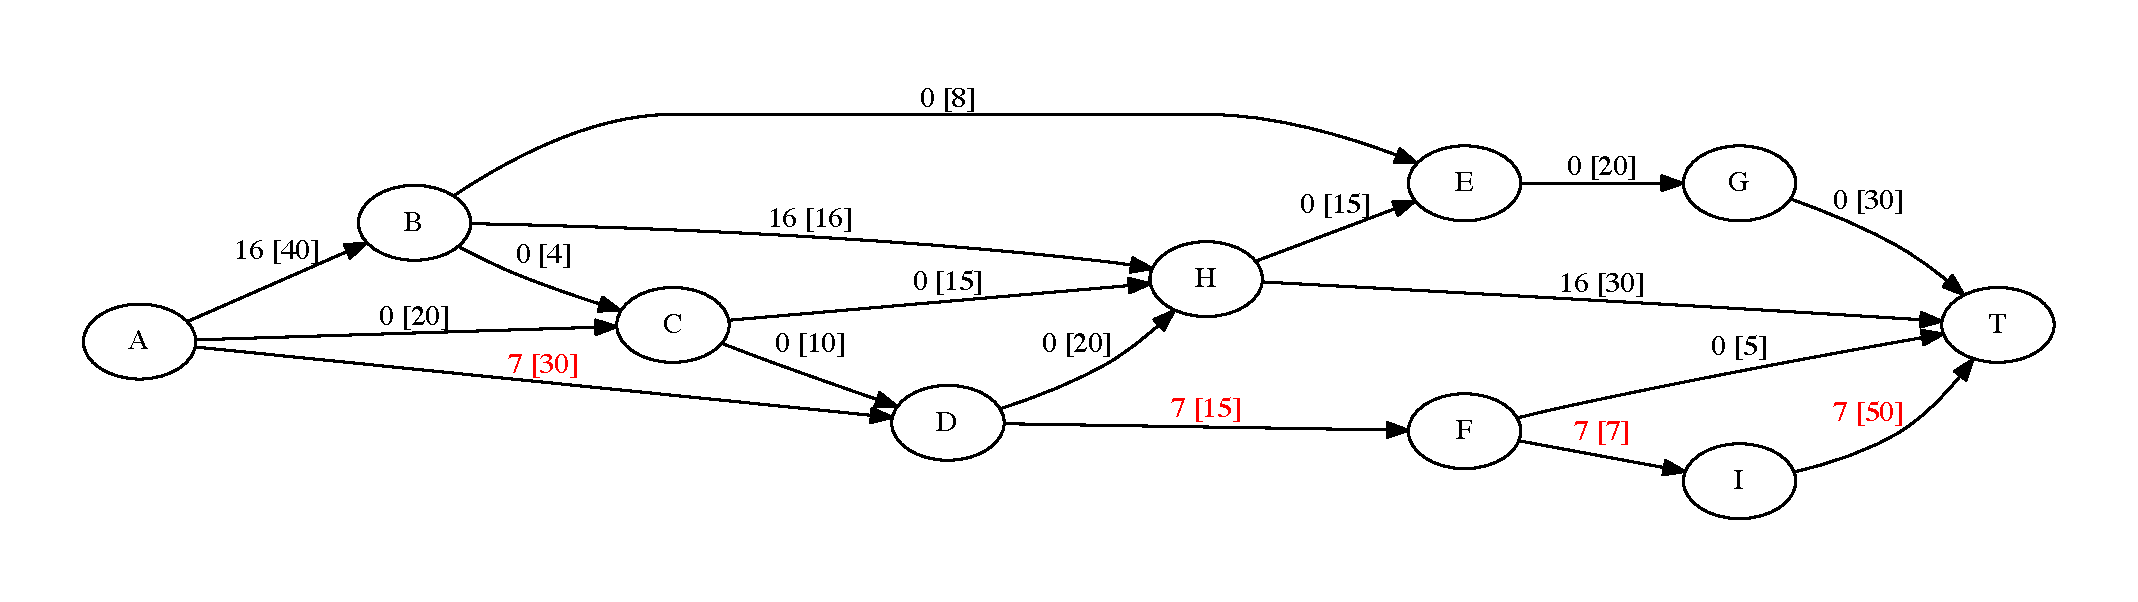
\includegraphics[width=\textwidth]{tutorials/pcc/figs/reseau-2.pdf}
    \end{center}
   
\end{frame}

\begin{frame}{}
    Troisième chaîne augmentante : A-B-E-G-T qui permet d'augmenter le flot de 8. 
    \begin{center}
        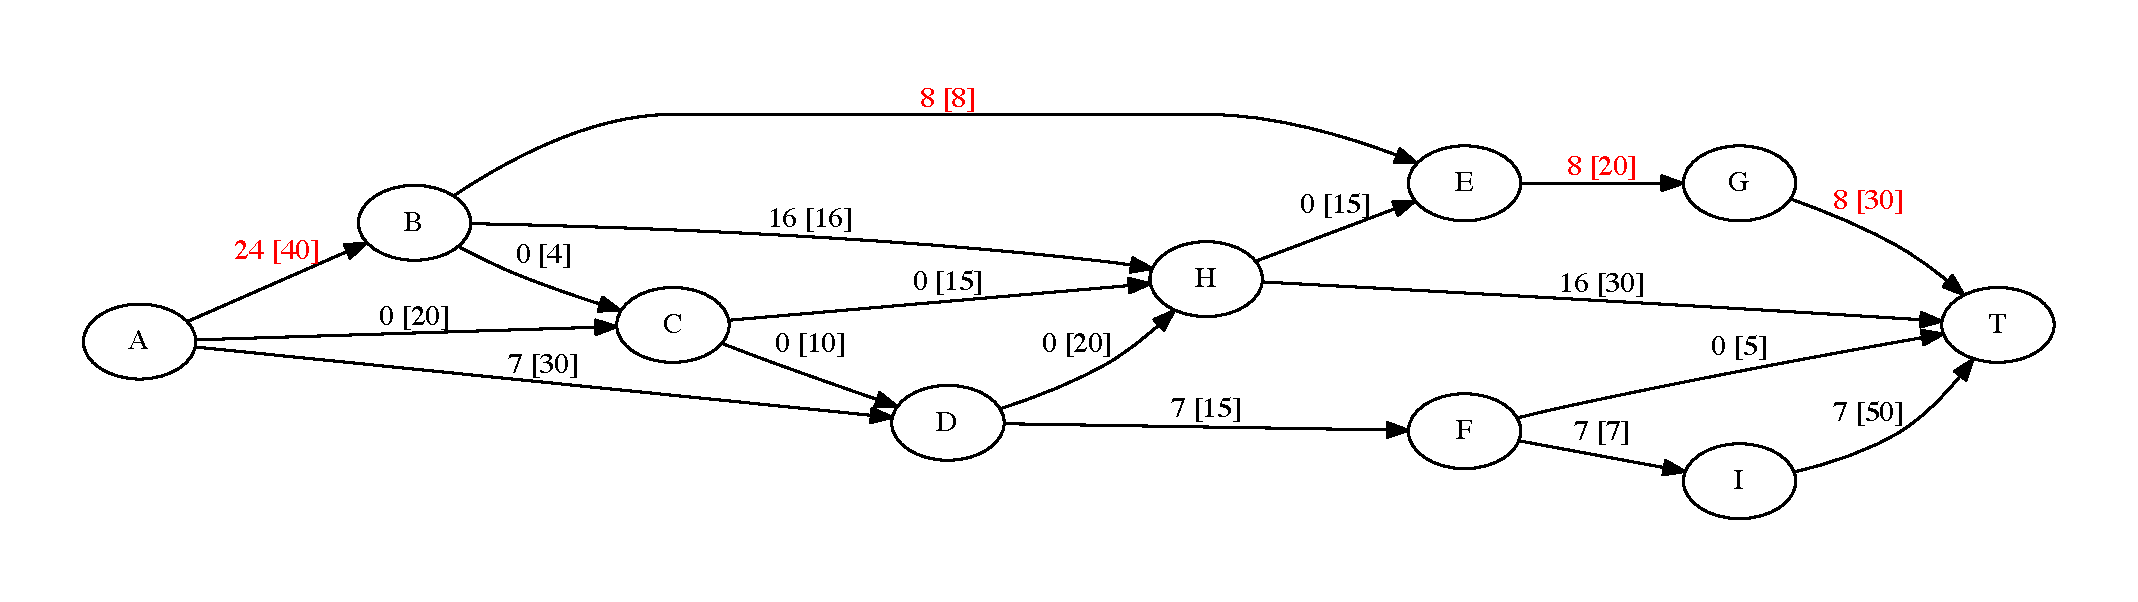
\includegraphics[width=\textwidth]{tutorials/pcc/figs/reseau-3.pdf}
    \end{center}
   
\end{frame}

\begin{frame}{}
    Quatrième chaîne augmentante : A-C-H-T qui permet d'augmenter le flot de 14.
    \begin{center}
        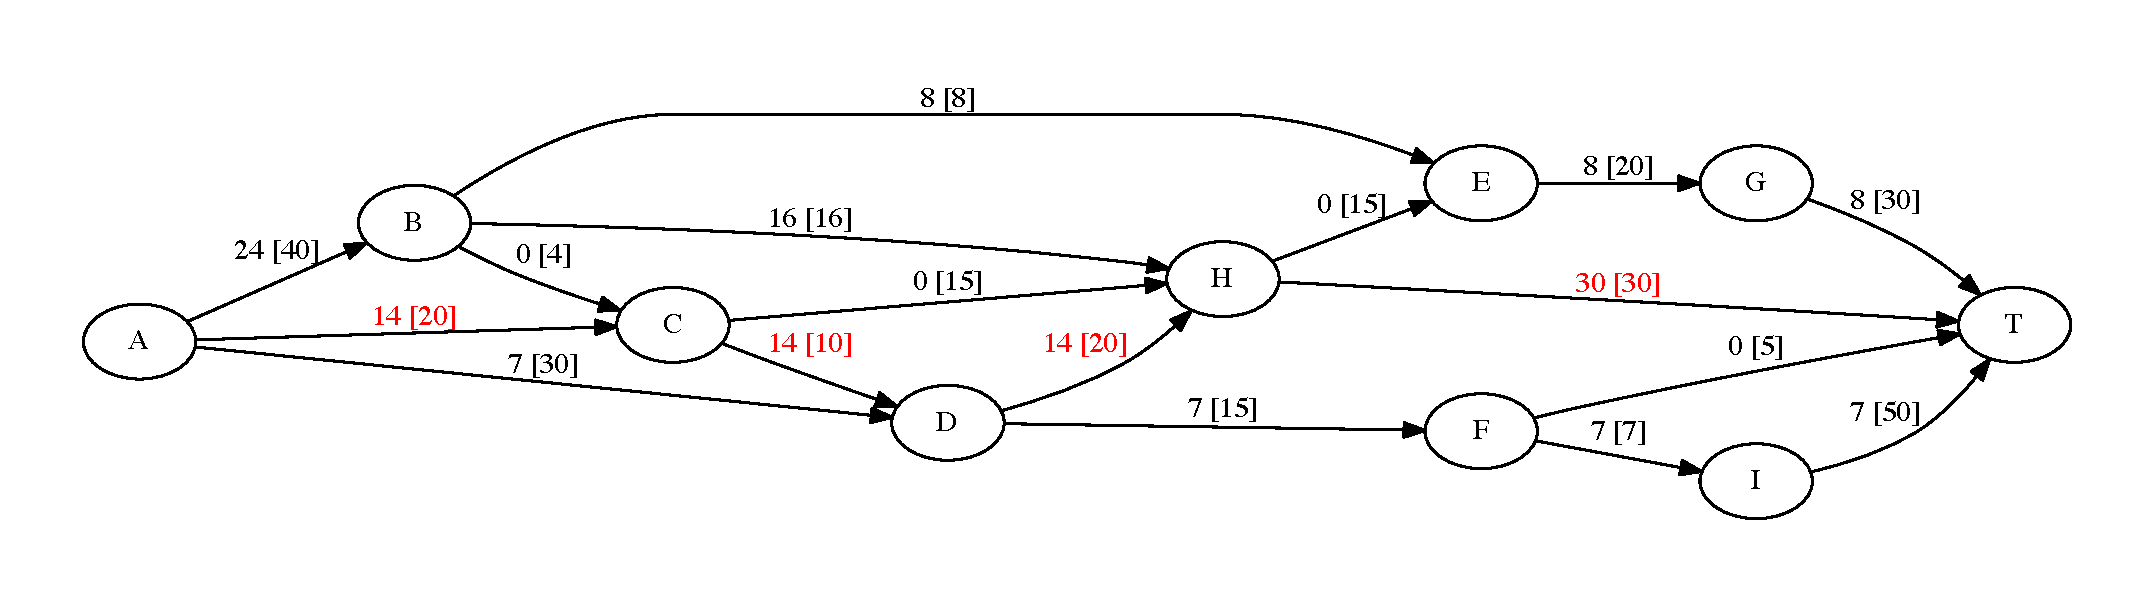
\includegraphics[width=\textwidth]{tutorials/pcc/figs/reseau-4.pdf}
    \end{center}
   
\end{frame}

\begin{frame}{}
    Le graphe devenant moins intuitif, on va appliquer l'algo de marquage.
    \begin{center}
        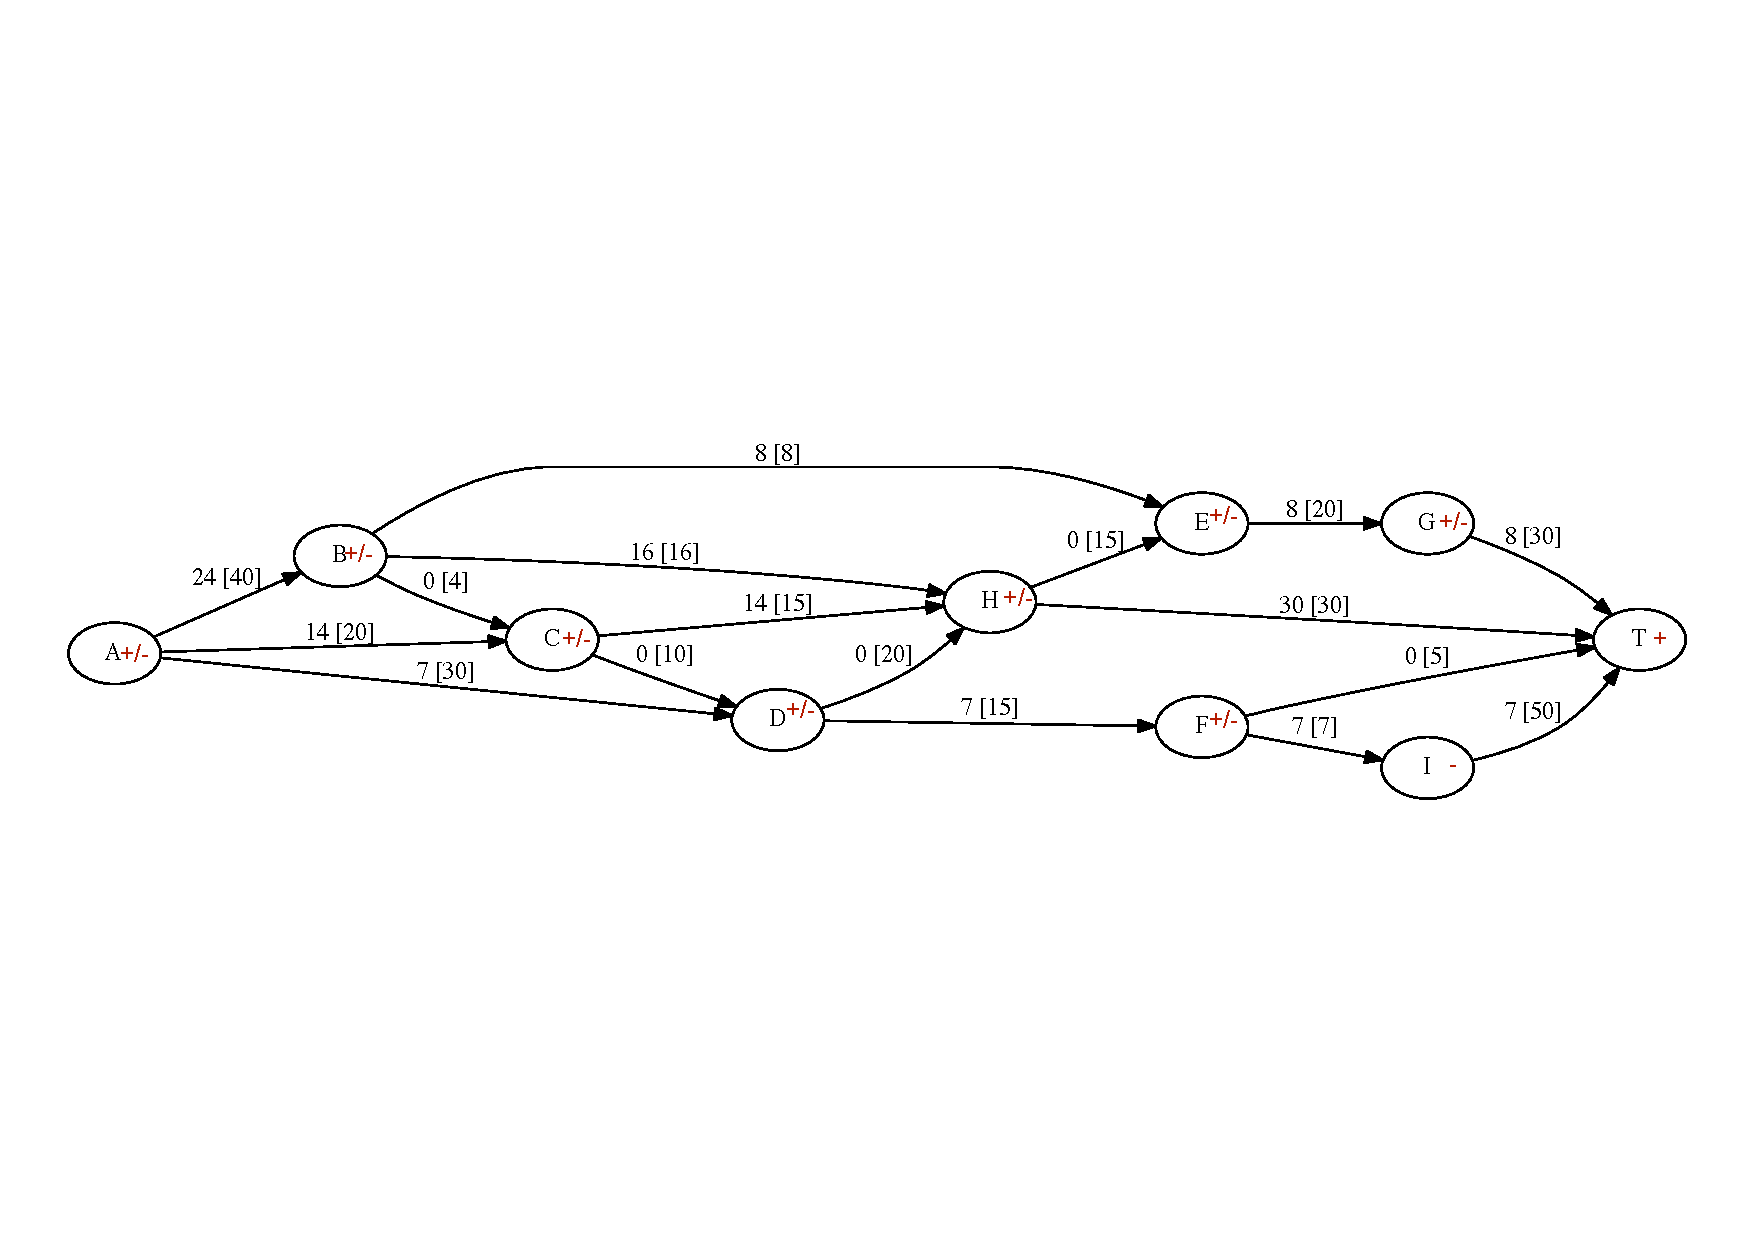
\includegraphics[width=\textwidth]{tutorials/pcc/figs/reseau-4m.pdf}
    \end{center}
   
\end{frame}

\begin{frame}{}
    Ce marquage permet de trouver une chaîne augmentante : A-D-H-E-G-T qui nous permet d'augmenter le flot de 12.
    \begin{center}
        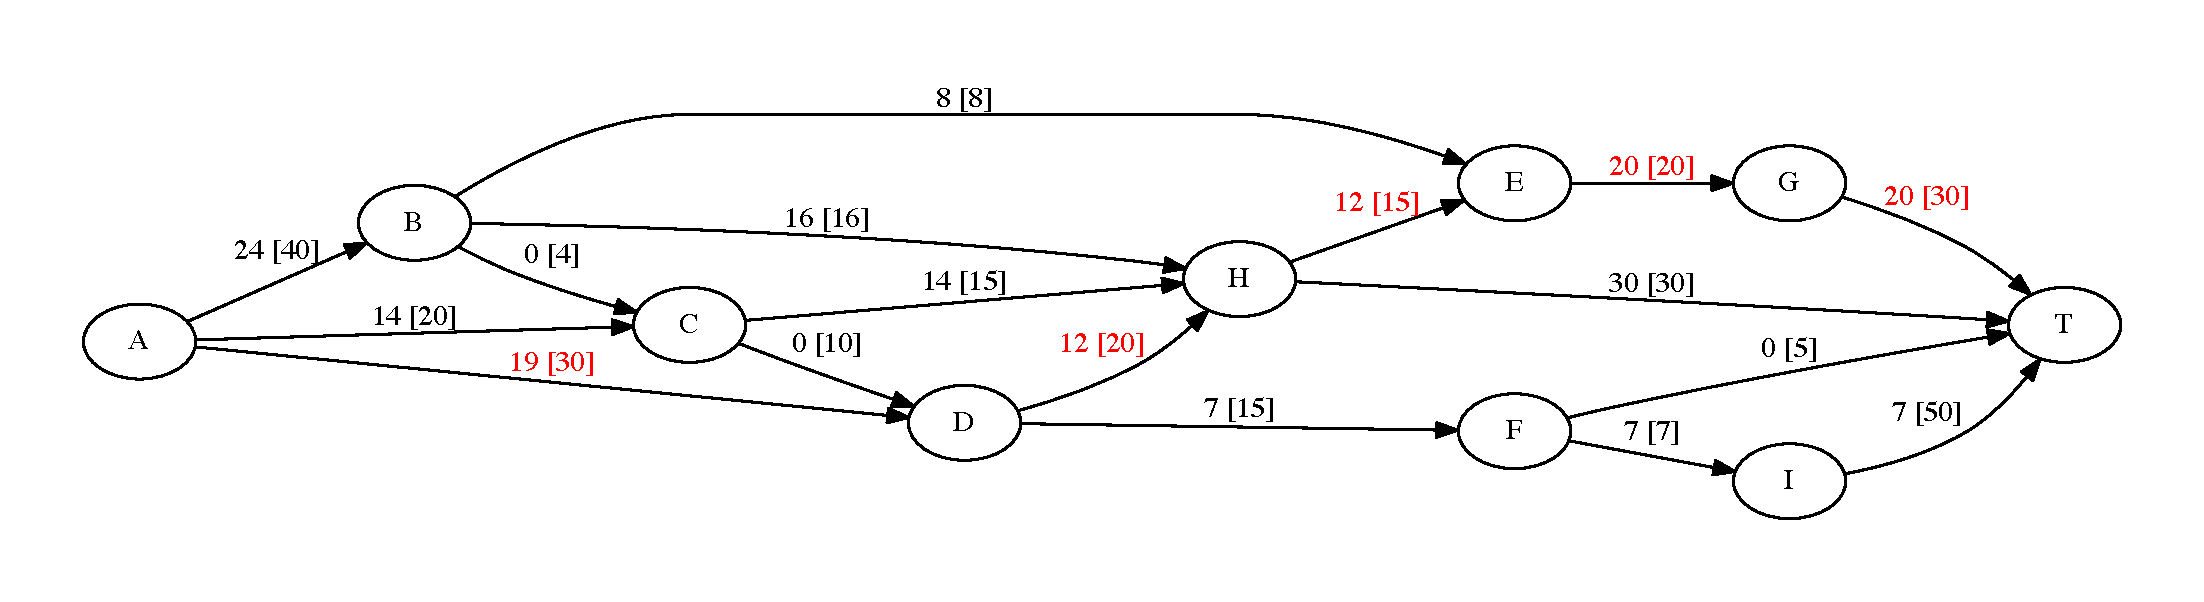
\includegraphics[width=\textwidth]{tutorials/pcc/figs/reseau-5.pdf}
    \end{center}
   
\end{frame}

\begin{frame}{}
    On recommence l'algorithme de marquage.
    \begin{center}
        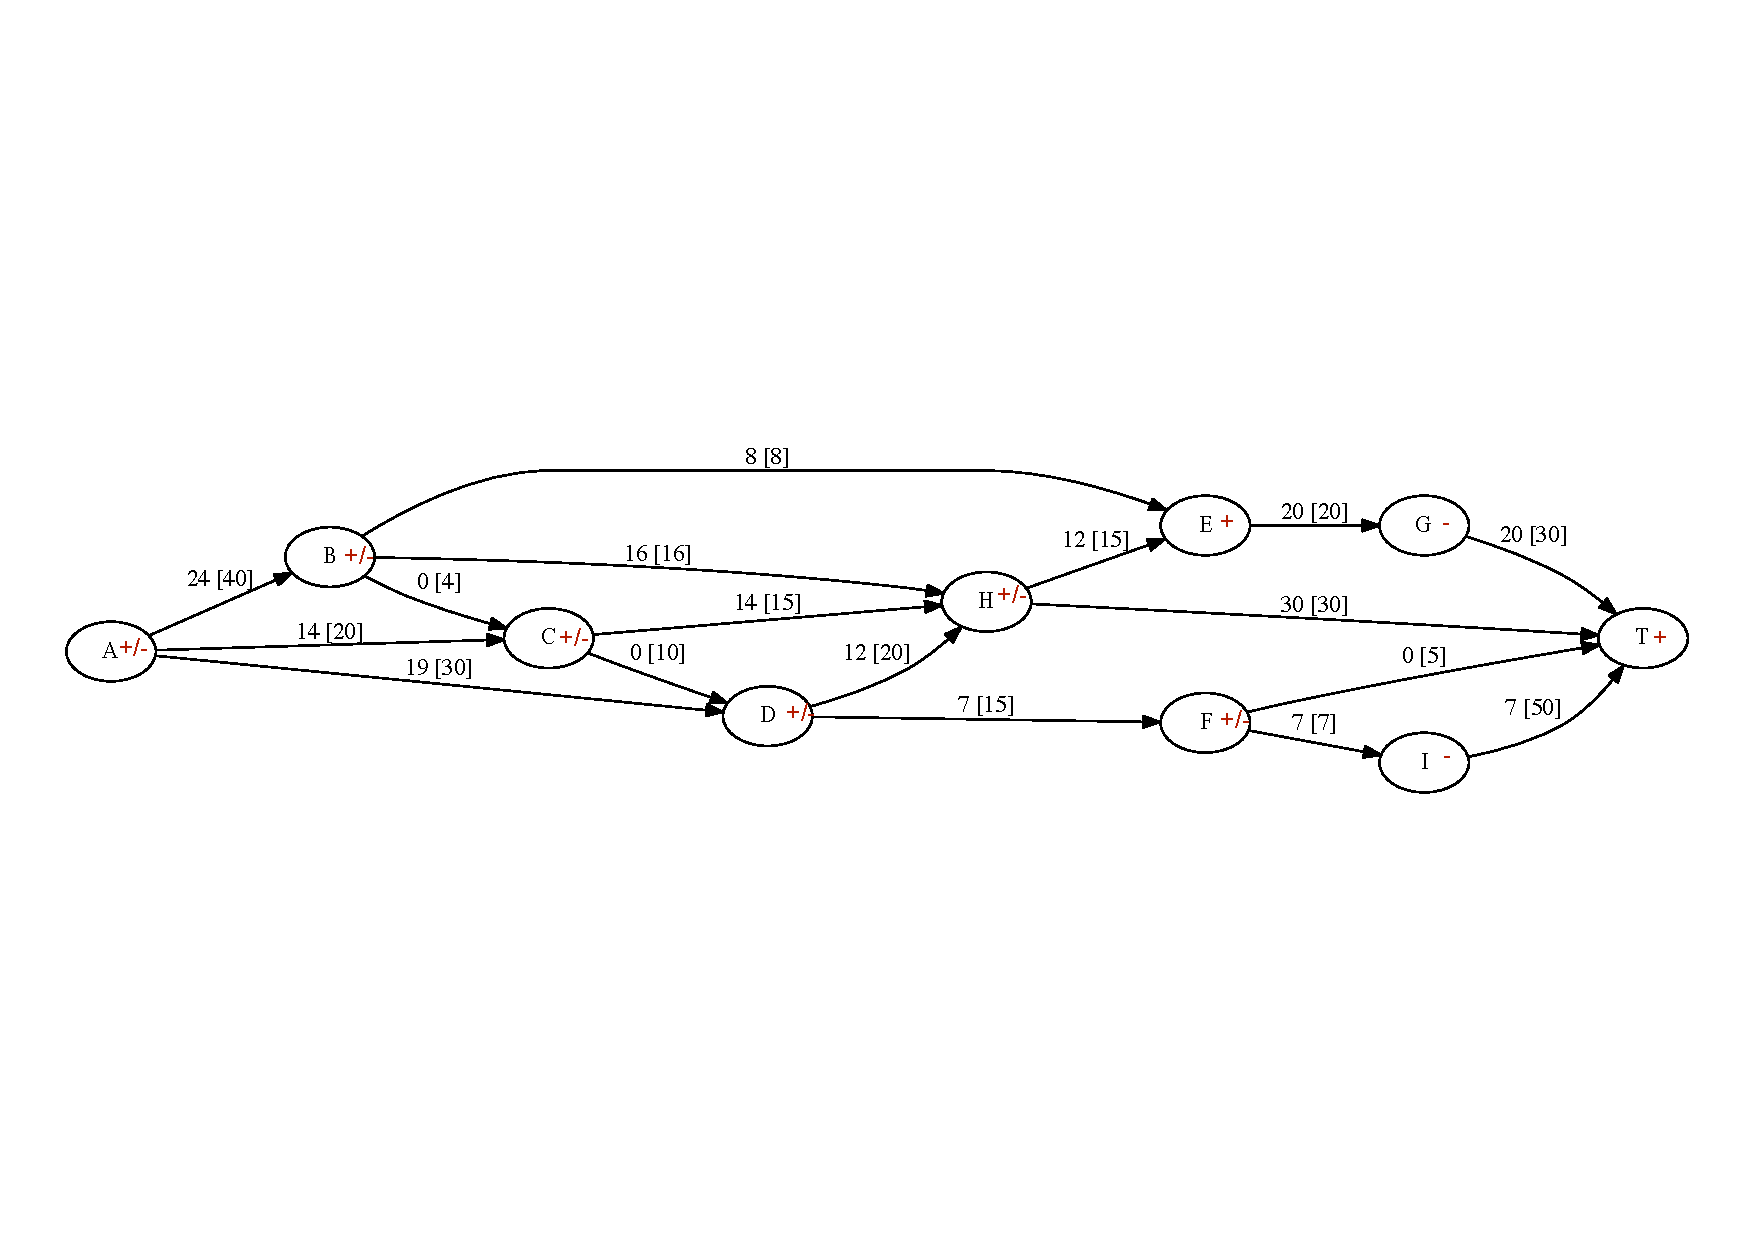
\includegraphics[width=\textwidth]{tutorials/pcc/figs/reseau-5m.pdf}
    \end{center}
   
\end{frame}

\begin{frame}{}
    Celui-ci nous donne une chaîne augmentante A-C-D-F-T qui permet d'augmenter le flot de 5.
    \begin{center}
        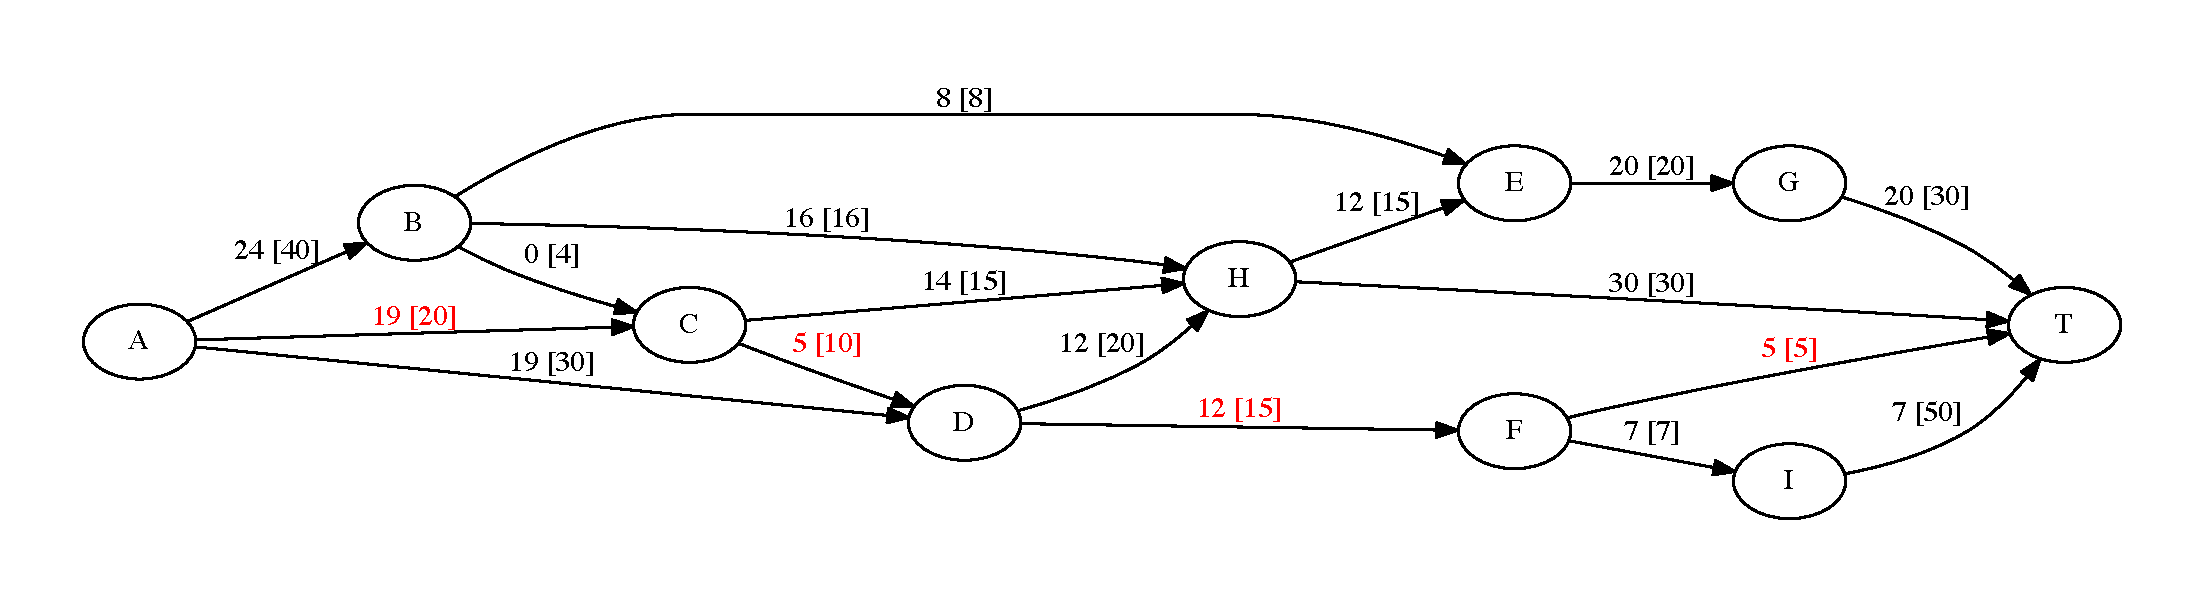
\includegraphics[width=\textwidth]{tutorials/pcc/figs/reseau-6.pdf}
    \end{center}
   
\end{frame}

\begin{frame}{}
    On ré-applique l'algorithme de marquage. Le sommet $T$ n'étant pas marqué +, l'algorithme est terminé. On vérifie en traçant la coupe, la capacité de celle-ci est de 62.

    \begin{center}
        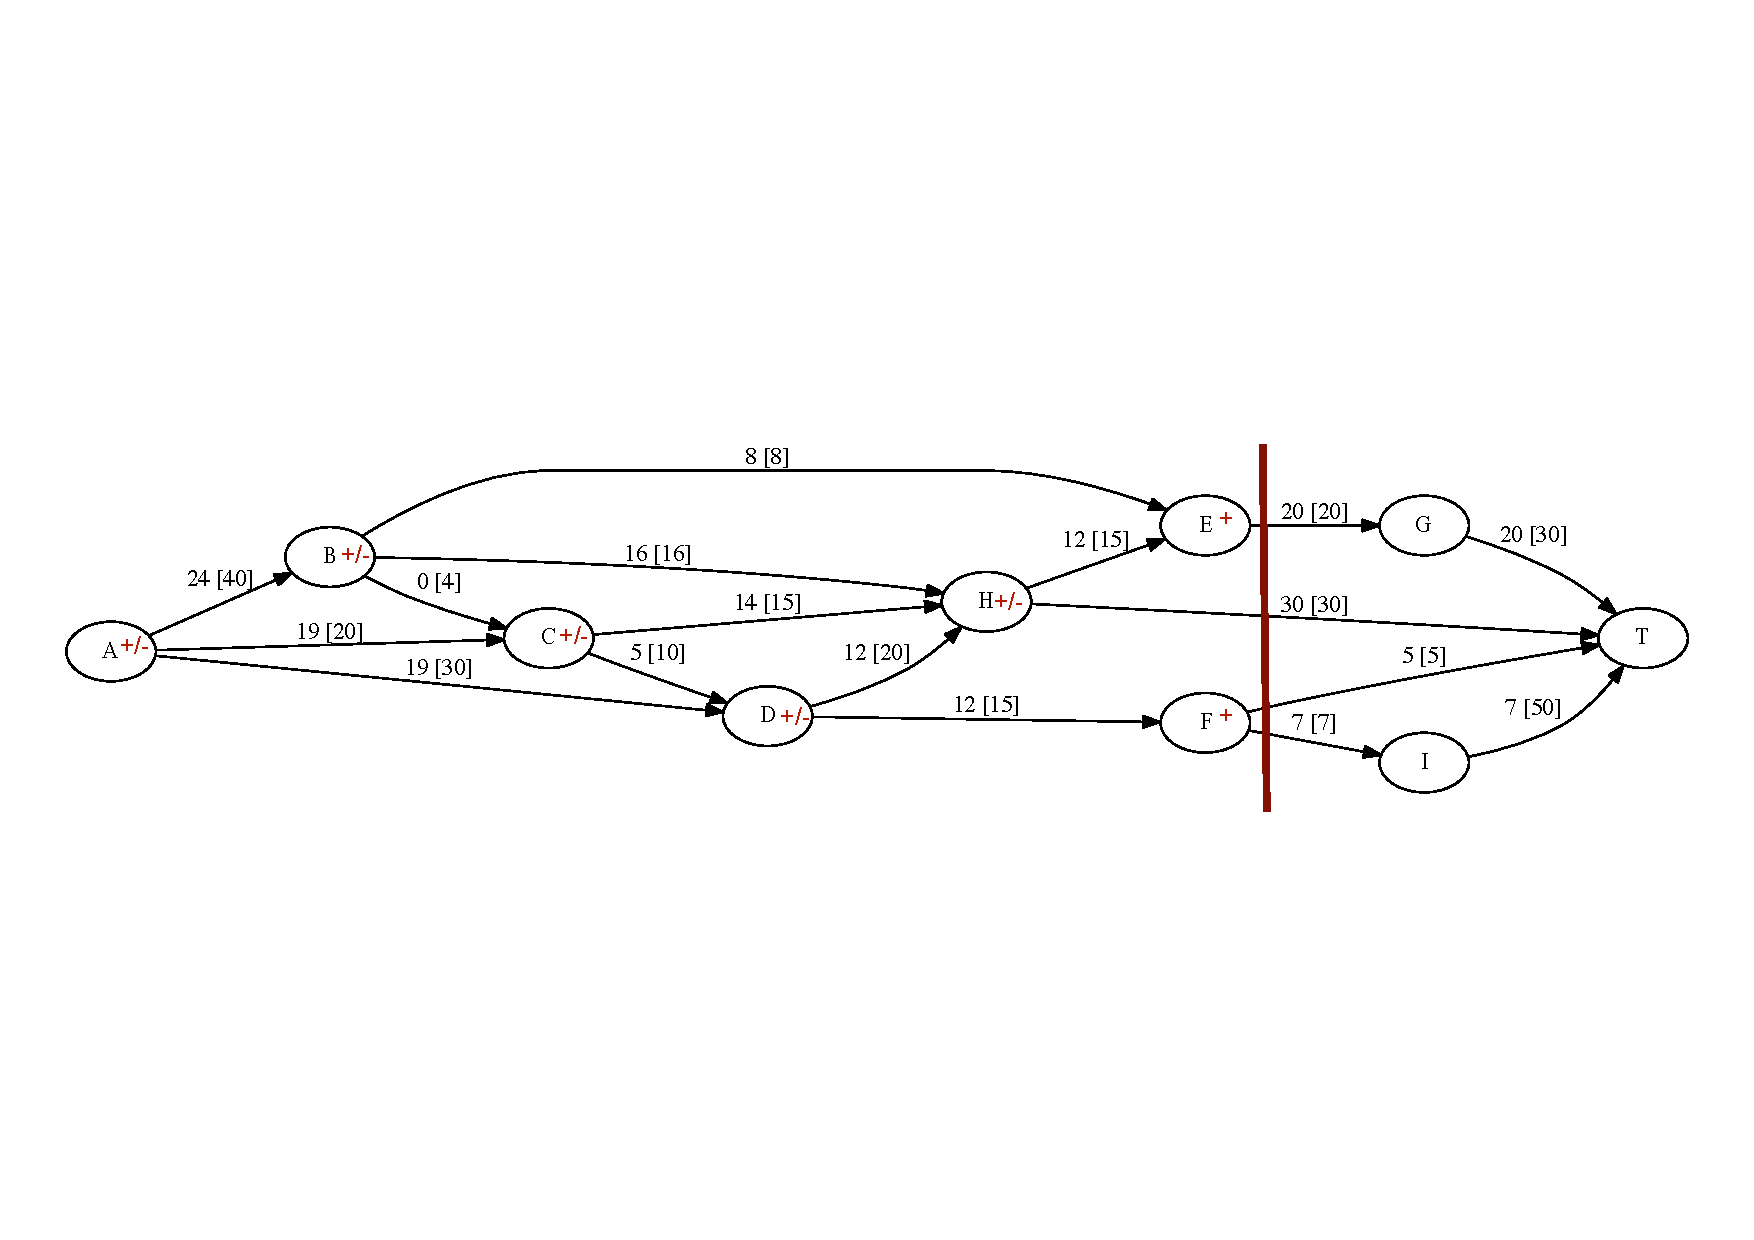
\includegraphics[width=\textwidth]{tutorials/pcc/figs/reseau-6m.pdf}
    \end{center}
   
\end{frame}


% flot max à cout min 
\section{Corrigé exercice flot max à coût min}
\begin{frame}{Modélisation}
    \begin{center}
        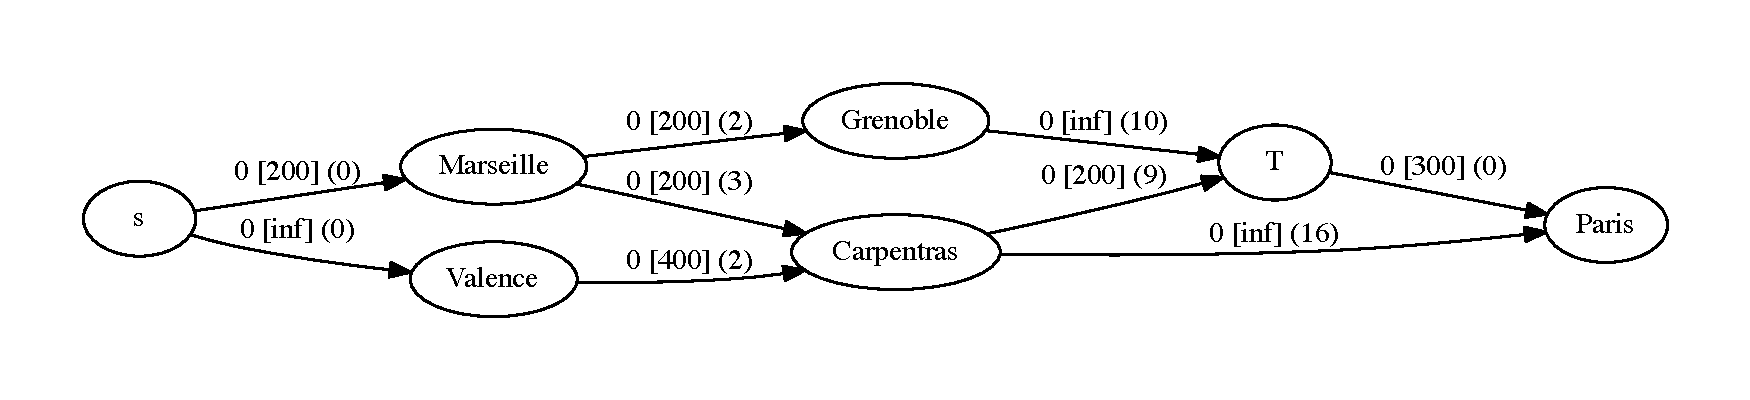
\includegraphics[width=\textwidth]{tutorials/flmcmin/fleurs-1.pdf}
    \end{center}
    Idée : train = 1 sommet supplémentaire
\end{frame}

\begin{frame}{Simplification}
    \begin{center}
        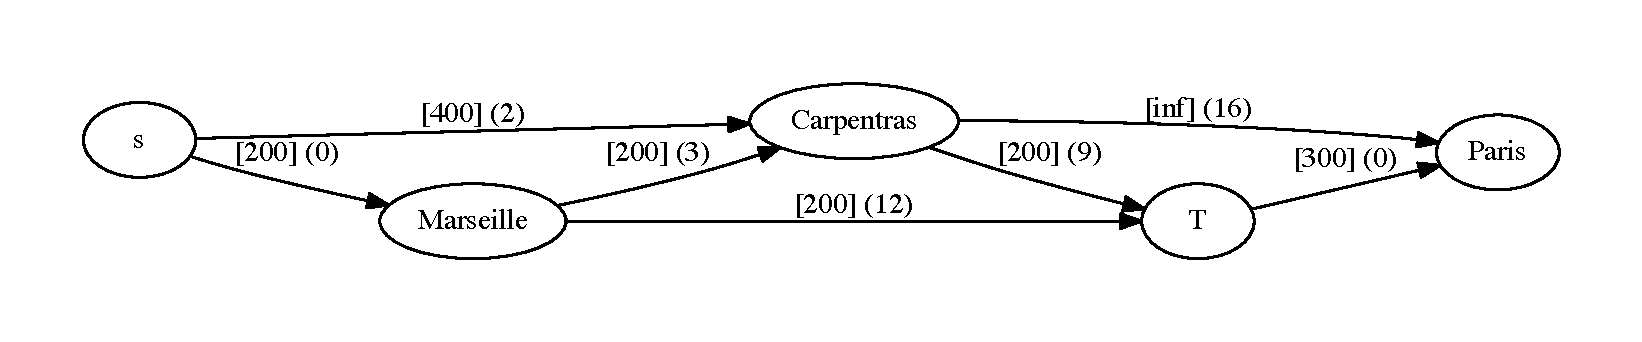
\includegraphics[width=\textwidth]{tutorials/flmcmin/fleurs-2.pdf}
    \end{center}
    Suppression des sommets Grenoble et Valence (loi de conservation)
\end{frame}



\begin{frame}{Résolution}
    Plus court chemin : s-Carpentras-T-Paris pour un coût de 11. On peut augmenter le flot de 200
    \begin{center}
        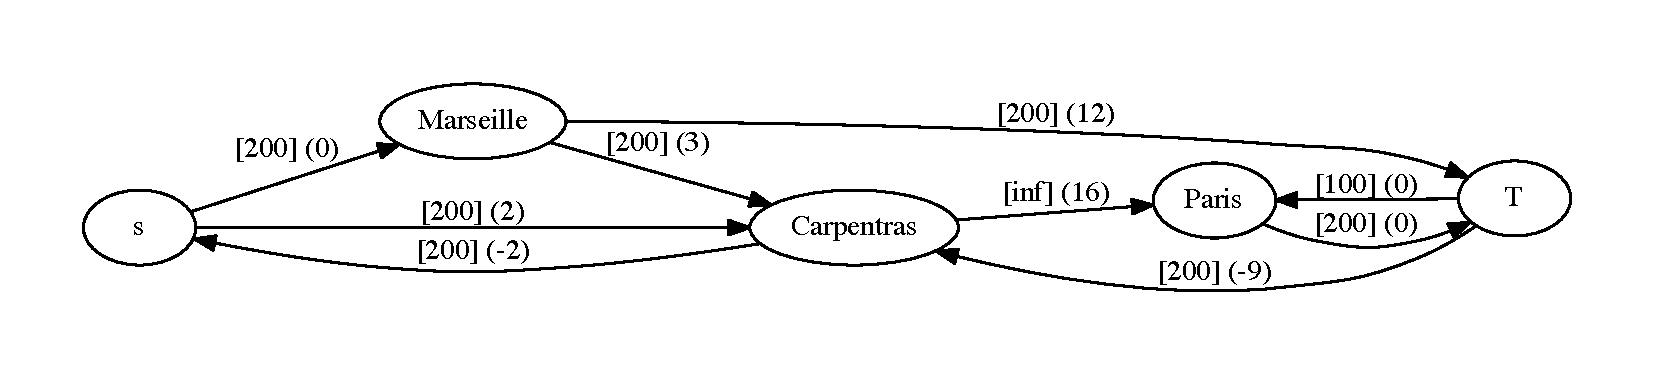
\includegraphics[width=\textwidth]{tutorials/flmcmin/fleurs-3.pdf}
    \end{center}
\end{frame}

\begin{frame}{Résolution}
    Plus court chemin : s-Marseille-T-Paris pour un coût de 12 et augmenter le flot de 100 à nouveau
    \begin{center}
        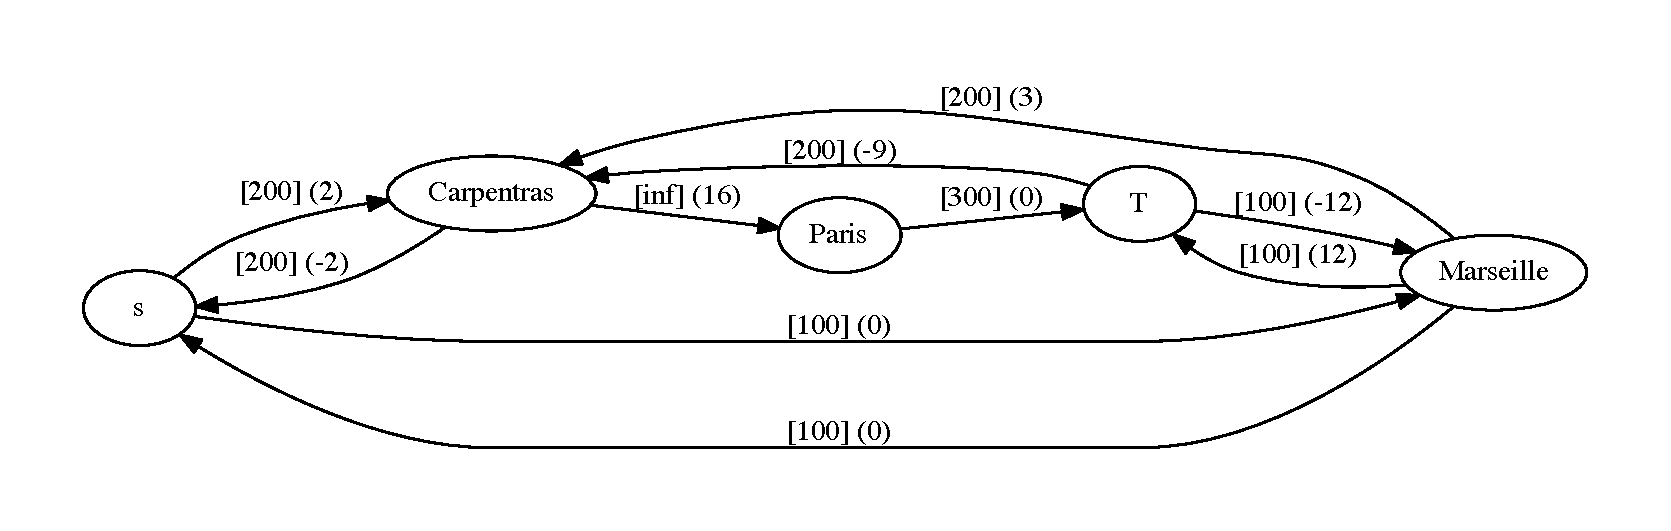
\includegraphics[width=\textwidth]{tutorials/flmcmin/fleurs-4.pdf}
    \end{center}
\end{frame}

\begin{frame}{Résolution}
    Plus court chemin : s-Carpentras-Paris qui a un coût de 18 et permet d'augmenter le flot de 200
    \begin{center}
        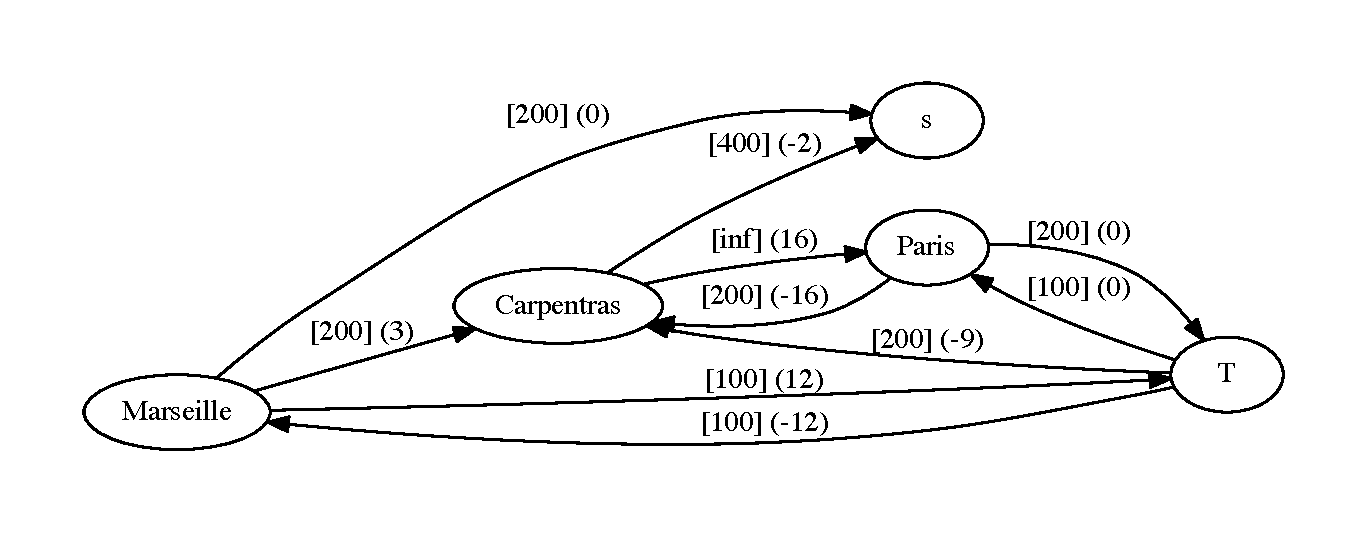
\includegraphics[width=\textwidth]{tutorials/flmcmin/fleurs-5.pdf}
    \end{center}
\end{frame}

\begin{frame}{Résolution}
    Dernier chemin possible : s-Marseille-Carpentras-Paris pour un coût de 19 et une augmentation de flot de 100.
    \begin{center}
        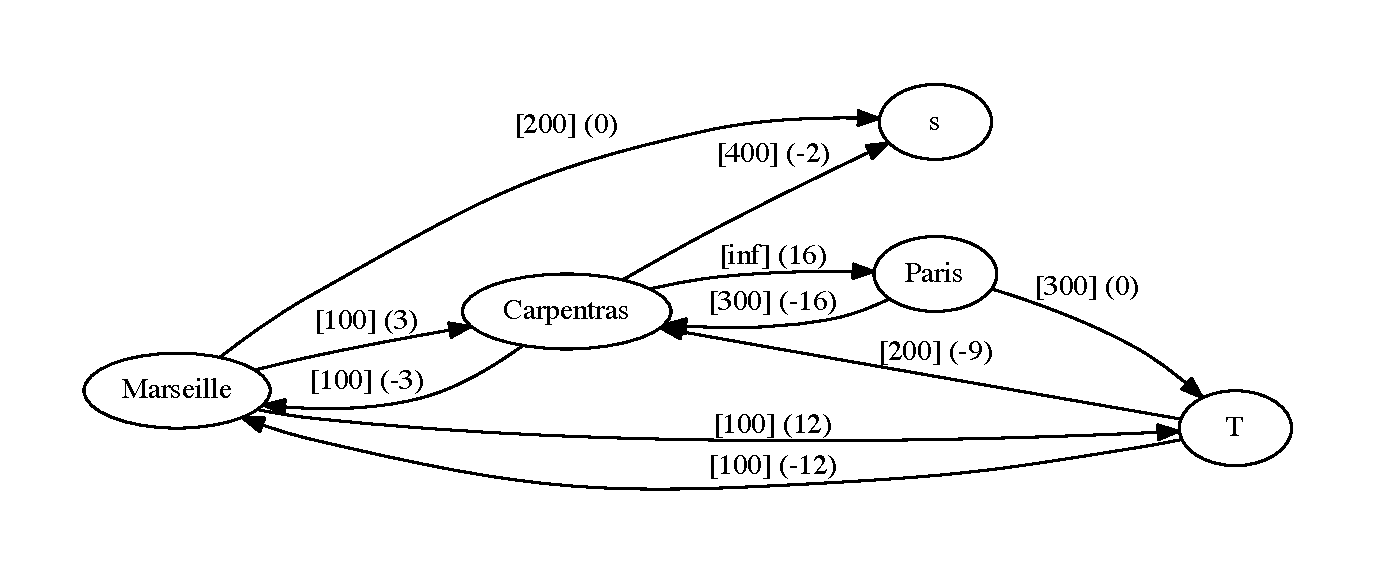
\includegraphics[width=\textwidth]{tutorials/flmcmin/fleurs-6.pdf}
    \end{center}
\end{frame}


\end{document}
